\documentclass[aspectratio=149]{beamer}


\usepackage{lmodern}
\usepackage{amsmath}
\usepackage{hyperref}
\usepackage{booktabs}
\usepackage{url}
\usepackage{smartdiagram}
\usepackage{bm}
\usepackage{csquotes}
\usepackage{graphicx}
\usepackage[utf8]{inputenc}
\usepackage{amsmath}
\usepackage{lipsum}
\usepackage{float}
\usepackage{textgreek}
\usepackage{tikz}
\usepackage{datetime}
\usepackage[backend=bibtex,style=authoryear]{biblatex}
\usepackage{listings}
\usepackage{setspace}
\usepackage{braket}
\usepackage[font=small,format=plain,labelfont=bf,up,textfont=normal,up,format=hang]{caption}

\usepackage{tikz}
\usetikzlibrary{shapes.geometric, arrows}

\usecolortheme{crane}

\tikzstyle{startstop} = [rectangle, rounded corners, minimum width=3cm, minimum height=1cm,text centered, draw=black, fill=red!30]
\tikzstyle{io} = [trapezium, trapezium left angle=70, trapezium right angle=110, minimum width=3cm, minimum height=1cm, text centered, draw=black, fill=blue!30]
\tikzstyle{process} = [rectangle, minimum width=3cm, minimum height=1cm, text centered, draw=black, fill=orange!30]
\tikzstyle{decision} = [diamond, minimum width=3cm, minimum height=1cm, text centered, draw=black, fill=green!30]
\tikzstyle{arrow} = [thick,->,>=stealth]

\addbibresource{refs.bib}

\newdateformat{monthyeardate}{\footnotesize \monthname[\THEMONTH], \THEYEAR}
\title{Face Detection, Recognition and Tracking}
\author[Pawan]{\texorpdfstring{\\}{}
    Pawan Singh Negi \- \texorpdfstring{$174010003$}{}  \texorpdfstring{\\}{}
    Aarif Shaikh \- \texorpdfstring{$173310007$}{}  \texorpdfstring{\\}{}
    M Kartheek \- \texorpdfstring{$163100065$}{}  \texorpdfstring{\\}{}
}

\institute[IITB]{Indian Institute of Technology, Bombay}


\begin{document}

\monthyeardate{}
\maketitle

%%%%%%%%%%%%%%%%%%%%%%%%%%%%%%%%%%%%

\begin{frame}
    \frametitle{Motivation}
    \begin{itemize}
        \item Something
    \end{itemize}
\end{frame}

%%%%%%%%%%%%%%%%%%%%%%%%%%%%%%%%%%%%

%%%%%%%%%%%%%%%%%%%%%%%%%%%%%%%%%%%%

\begin{frame}
\frametitle{Motivation}
\begin{itemize}
	\item something
\end{itemize}
\end{frame}

%%%%%%%%%%%%%%%%%%%%%%%%%%%%%%%%%%%%

\begin{frame}
\frametitle{Overall flow of the Process}
\begin{figure}
	\centering
	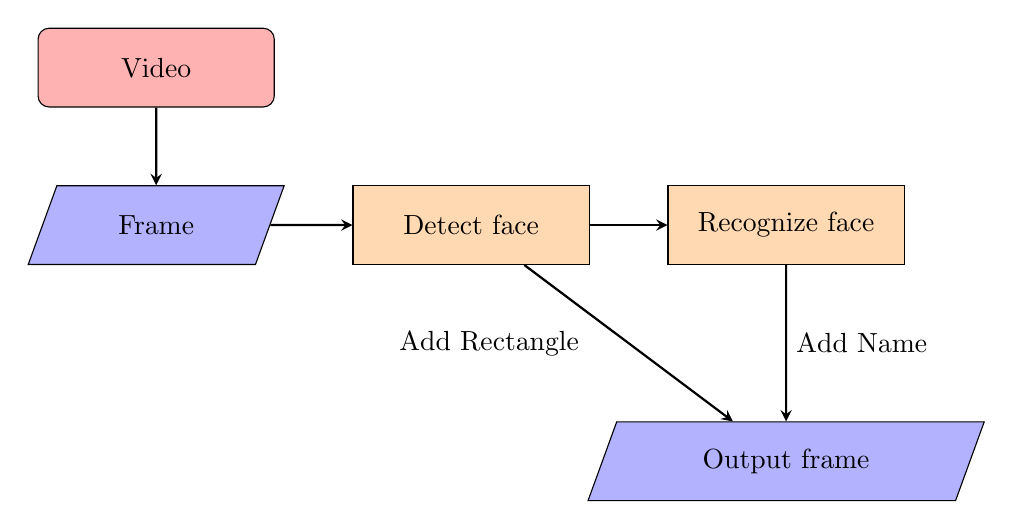
\begin{tikzpicture}[node distance=2cm]
	
	\node (start) [startstop] {Video};
	\node (frame) [io, below of=start] {Frame};
	\node (detect) [process, right of=frame, xshift=2cm] {Detect face};
	\node (recognize) [process, right of=detect, xshift=2cm] {Recognize face};
	\node (outframe) [io, below of=recognize , yshift=-1cm] {Output frame};
	
	\draw [arrow] (start) -- (frame);
	\draw [arrow] (frame) -- (detect);
	\draw [arrow] (detect) -- (recognize);
	\draw [arrow] (detect) -- node[anchor=east , xshift=-0.5cm] {Add Rectangle} (outframe);
	\draw [arrow] (recognize) -- node[anchor=west] {Add Name} (outframe);
	
	\end{tikzpicture}
	\caption{Flowchart}
\end{figure}
	
\end{frame}

%%%%%%%%%%%%%%%%%%%%%%%%%%%%%%%%%%%%

\begin{frame}
    \centering
    Thank you
\end{frame}

\begin{frame}[t,allowframebreaks]
  \frametitle{References}
  \printbibliography{}
\end{frame}


%%%%%%%%%%%%%%%%%%%%%%%%%%%%%%%%%%%%

\end{document}
%%% Local Variables:
%%% mode: latex
%%% TeX-master: t
%%% End:
